%!TEX root = nextndnvideo-tr.tex
\section{implementation} % (fold)
\label{sec:implementation}
NDNlive and NDNtube are developed using Consumer / Producer API and Gstreamer 1.4.3 library.\footnote{Other versions of Gstreamer may not be compatible}
The supported platforms are Mac OS X and Linux Ubuntu.\footnote{Other Linux platforms are potentially supported} 

\subsection{NDNlive}
As shown in Figure~\ref{fig:NDNlive_arch}, NDNlive consists of two applications --- one is running at the publisher's host and another one at the consumer's host. In this section, we go over implementation details of the publisher's application and then continue with consumer's application.

\begin{figure*}%[htbp]
  \centering
  \includegraphics[scale=0.3]{NDNlive_naming_pro}
  % \vspace{-0.3cm}
  \caption{Locations of producers and consumers in the NDNlive namespace.}
  \label{fig:NDNlive_cp}
  %\vspace{-0.2cm}
\end{figure*}

\subsubsection{Publisher}
\label{ssub:NDNlive_pro}
Publisher's application has four producers: video content producer, video stream information producer, audio content producer and audio stream information producer. Figure~\ref{fig:NDNlive_cp} shows the locations of the producers in the NDNlive namespace. 

Two content\_producers continuously publish video and audio frames by incrementally increasing the correpsonding frame numbers (Figure~\ref{fig:NDNlive_naming}). 

Two stream\_info producers continuously publish up-to-date information about the live streaming media: current frame number, frame rate, video width and height, encoding format (Figure~\ref{fig:NDNlive_naming}).

\paragraph{Negative Acknowledgement} % (fold)
\label{par:negative_acknowledgement}
\vspace{0.3cm}
In some situations, the live stream publisher is not able to satisfy Interests with actual data (e.g. video and audio frames).

\begin{enumerate}
	\item The consumer may sometimes miscalculate the pacing of video and audio frames and request the frame that does not exist at the moment (e.g. ahead of the production). The publisher can inform the consumer about this situation using \textit{nack()} function of the Consumer~/~Producer API. 

	As illustrated by the Algorithm~\ref{alg:liveproducer}, producer calls \textit{nack()} function with \textit{PRODUCER\_ \\\ DELAY} header containing the anticipated time value after which the data may become available.

	But in our latest implementation, we remove this part because we finally decide keeping some outstanding interests to leverage the delay between producer and consumer. So if the producer meets interest requesting for the data which are not yet produced, it will just omit these interest. Such interests will be satisfied later from the producer's \textit{Send\_Buffer}. We will discussion this in more details in Section~ \ref{par:consume_interval_pipelining}.
	
	\item Consumers join the live stream after the publisher. Since the publisher of the live stream stores only a limited number of the most recently produced audio and video frames, some consumers might request the frames that has already expired everywhere in the network. In this case, the publisher calls the \textit{nack()} operation with \textit{NO-DATA} header, which informs consumers that a particular video or audio frame is no longer available.
	
\end{enumerate}
% paragraph negative_acknowledgement (end)

The pseudocode of NDNlive publisher application is provided in Algorithm~\ref{alg:liveproducer}.

\begin{algorithm}[ht]
\caption{NDNlive producer}
\label{alg:liveproducer}
\begin{algorithmic}[1]
\State $h_v \leftarrow $ \textbf{producer}(/ndn/ucla/NDNlive/stream-1/video/ \\\ content)
\State \textbf{setcontextopt}($h_v$, \textbf{cache\_miss}, \textit{ProcessInterest})
\State \textbf{attach}($h_v$)
\vspace{0.2cm}
	\While{\textit{TRUE}}
	\State $Name \textbf{ } suffix_v \leftarrow $ video frame number
	\State $content_v \leftarrow $ video frame captured from camera
	\State \textbf{produce}($h_v$, $Name\textbf{ }suffix_v$, $content_v$)
	\EndWhile
\vspace{0.2cm}
\vspace{0.2cm}
\State $h_a \leftarrow $ \textbf{producer}(/ndn/ucla/NDNlive/stream-1/audio/ \\\  content)
\State \textbf{setcontextopt}($h_a$, \textbf{cache\_miss}, \textit{ProcessInterest})
\State \textbf{attach}($h_a$)
\vspace{0.2cm}
	\While{\textit{TRUE}}
	\State $Name \textbf{ } suffix_a \leftarrow $ audio frame number
	\State $content_a \leftarrow $ audio frame captured from mirophone
	\State \textbf{produce}($h_a$, $Name\textbf{ }suffix_a$, $content_a$)
	\EndWhile
\vspace{0.4cm}
\Function{ProcessInterest}{Producer \textbf{h}, Interest \textbf{i}}
  \If{\textit{NOT Ready}}
    \State $appNack \leftarrow $ \textbf{AppNack}($i$, \textbf{RETRY-AFTER})
    \State \textbf{setdelay}($appNack$, $estimated\_time$)
    \State \textbf{nack}($h$, $appNack$)
  \EndIf
   \If{\textit{Out of Date}}
    \State $appNack \leftarrow $ \textbf{AppNack}($i$, \textbf{NO-DATA})
    \State \textbf{nack}($h$, $appNack$)
  \EndIf
\EndFunction
\end{algorithmic}
\end{algorithm}

\begin{algorithm}[hbt]
\caption{NDNlive consumer}
\label{alg:liveconsumer}
\begin{algorithmic}[2]
\State $h_v \leftarrow $ \textbf{consumer}(/ndn/ucla/NDNlive//stream-1/video/\\\ content, \textit{UDR})
%\State \textbf{setcontextopt}($h_v$, \textit{EMBEDDED\_MANIFESTS}, \textit{TRUE})
%\State \textbf{setcontextopt}($h_v$, \textbf{receive\_buffer\_size}, 1MB)
\State \textbf{setcontextopt}($h_v$, \textbf{new\_segment}, \textit{ReassambleVideo})
\vspace{0.2cm}
	\While{\textit{reaching Video\_Interval}}
	\State $Name \textbf{ } suffix_v \leftarrow $ video frame number
	\State \textbf{consume}($h_v$, $Name\textbf{ }suffix_v$)
	\State $framenumber ++$
	\EndWhile
\vspace{0.2cm}

\Function{ReassembleVideo}{Data \textbf{segment}}
    \State $content \leftarrow $ reassemble \textbf{segment}
    \If{\textit{Final\_Segment}}
		\State $video \leftarrow $ decode \textbf{content}
	   	\State Play $video$
	\EndIf
\EndFunction

\vspace{0.4cm}

\State $h_a \leftarrow $ \textbf{consumer}(/ndn/ucla/NDNlive/stream-1/audio/\\\ content, \textit{SDR})
\State \textbf{setcontextopt}($h_a$, \textbf{new\_content}, \textit{ProcessAudio})
\vspace{0.2cm}
	\While{\textit{reaching Audio\_Interval}}
	\State $Name \textbf{ } suffix_a \leftarrow $ audio frame number
	\State \textbf{consume}($h_a$, $Name\textbf{ }suffix_a$)
	\State $framenumber ++$
	\EndWhile
\vspace{0.2cm}

\Function{ReassembleAudio}{Data \textbf{content}}
%   \State $video \leftarrow $ decode \textbf{content}
   	\State $audio \leftarrow $ decode \textbf{content}
   	\State Play $audio$
\EndFunction
\end{algorithmic}
\end{algorithm}

\subsubsection{Player}
\label{ssub:NDNlive_con}
NDNlive consumer must fetch the live stream information to set up the Gstreamer playing pipeline before it can request any of the audio or video frames. The application has four consumers: video content consumer, video stream information consumer, audio content consumer and audio stream information consumer. 

\paragraph{Data retrieval}
\label{par:NDNlive_dataretrievalprotocol}
\vspace{0.3cm}
Consumer / Producer API protocol suite offers three data retrieval protocols: SDR, UDR, RDR. In this section we describe how NDNlive consumer application uses SDR and UDR (the latest implementation, we use RDR instead of UDR) protocols. The pseudocode of the NDNlive consumer application is provided in the Algorithm~\ref{alg:liveconsumer}. 

\begin{enumerate}
	\item {\textit{Content Retrieval}}
	
In the case of the live media streaming, the consumer application must continue retrieving video and audio frames at all times in order to keep up with the data production rate. All segments of each frame must be retrieved as fast as possible and the fetching process should not block other frames because of segment losses. 

NDNlive audio content consumer uses \textbf{SDR} (\textit{Simple Data Retrieval}) for audio frame retrieval. UDR does not pipeline Interest packets, which satisfies our requirements, since the audio frame is small enough to fit in just one Data segment.	

NDNlive video content consumer uses \textbf{UDR} (\textit{Unreliable Data Retrieval}) protocol for video frame retrieval. Since \textbf{UDR} pipelines Interests transmission and does not provide ordering, some Data segments may arrive out of order. NDNlive consumer application takes care of Data segment reassembly and drops the whole frame is any of its segments are lost. 

But after several months' developments, we have switched NDNlive video data retrieval protocol from \textbf{UDR} to \textbf{RDR}, and audio data from \textbf{SDR} to \textbf{RDR}. The reasons are as following:
	\begin{enumerate}
		\item One video frame is often consisted of several segments (1 - 25). If one segment is missing, the whole frame will be useless. If we don't do retransmission for that segment, the other segments retrieved are wasted. And the accumulation of missing frames will cause synchronization problem between audio and video. And we found that segment missing is common, so we need retransmission.
		\item If one interest arrived at producer side ahead of time, but in the reality it is very hard for the producer to estimate the Retry-After time of NACK. If this time is too small, the NACK is meaningless, because the next interest requesting the same segment is still not generated. If this time is too big, it will cause the delay of data retrieval, which we could not like see, neither. In the real experiments, we observe that if we could set the appropriate TIME-OUT and Retransmission-Time threshold for each interest and also the frame pipelining window, we could solve the problem of interests arriving too early or even make a good use of it: There could be always some outstanding interests(the number is controlled by the frame pipelining window) which will arrive at the producer part before they are generated. They would not be satisfied when they just arrived, but will be satisfied right away when the corresponding data are generated. For example, the video generating rate is 30 per second. It means that every 33 milliseconds, one video frame will be generated. What's more, the average RTT is 50 milliseconds, then one segment will arrive at the consumer side after 25 milliseconds. Then We could save at least half of the RTT compared to using Retry-After NACK, and the delay will also be leveraged or even eliminated. If the data was not retrieved within the lifetime, the retransmission will be issued and will be controlled by the threshold. We will discuss the frame pipelining fetching in more detail in the Fetching Pipelining paragraph. The point is that we need retransmission feature for both video and audio. 
		\item We need to do reordering and reassembling if we use UDR. But RDR will help us do these. It's another benefit of RDR.
	\end{enumerate}
So after many experiments and considerations, we finally adopted RDR instead of UDR/SDR for NDNlive content retrieval. It doesn't mean that UDR is of no use, but RDR suits more according to such situations. We still keep the old design description to show the whole development curve. We want to share the designing path of NDNlive and hope this also will give other NDN APP developers some inspirations. We also don't change the PseudoCode of NDNlive(UDR version), because it shows that how people could use UDR and NACK. The pseudocode of the latest version of NDNlive using RDR looks almost the same with the NDNtube, which will be shown in next section. Because of the complexity of frame pipelining of consumer side and the playing back of producer side, the pseudocode will only show the parts related to the Consumer/Producer API.

	\item {\textit{Stream Information Retrieval}} 
	
Stream information is periodically updated by the video publisher, which essentially means creation of a new Data packet with a unique name (e.g. new timestamp name component). The consumer that is trying to join the live stream does not know the unique name of the latest stream information object, and therefore cannot use UDR or RDR protocols which assume such knowledge. A simple solution of this problem is to use  \textbf{SDR} (\textit{Simple Data Retrieval}) protocol with \textit{Right\_Most\_Child} option set as TRUE. The protocol generates a single Interest packet with \textit{RightmostChildSelector} which is capable of fetching the latest stream info object. 

\end{enumerate}
\vspace{-0.5cm}

\paragraph{Frame-to-frame Interval and Fetch Pipelining}
\vspace{0.1cm}
\label{par:consume_interval_pipelining}
Consumer application should control the Interest sending speed. If it sends Interests too aggressively and the data is not yet produced by the publisher application, the playback may collapse. If it sends Interests too slowly, the playback may fall behind the video generation. NDNlive uses constant frame rate encoding, therefore for a video, which is encoded by 30 frames per second, the interval between frames is $1000/30 \approx {33.3}$ millisecond. In other words, if the next frame can't be retrieved within 33 ms, the playing back will be sucked. As we discussed above, now we use RDR to retrieve every frame. 

RDR will handle the reordering and reassembling inside one frame and also the retransmission for us. But we need do the pipelining between frames. Our strategy is to set up a 
\textit{Pipeline\_Window} which will be adjusted automatically according to the real-time RTT. The amount of frames which will be sending at the same time is equal to \textit{Pipeline\_Window} size. Any finished frame will trigger the following one frame. For example, now frame 13 to frame 22 is under retrieval, and frame 12 is just finished(may before frame 10), frame 23 will be issued immediately. So we should do the reordering inside the window. 

\textit{Pipeline\_Window} can be calculated according to \textit{Frame\_RTT}: 

$Pipeline\_Window =  Frame\_RTT / (1000 / FrameRate) $ 

$Frame\_RTT = Accumulating\_Time / Frame\_Numbers$

So the \textit{Frame\_RTT} here is referring to the average retrieving time of one frame. This formula can be understood very straightforwardly. If the frame retrieving speed wants to match the generating speed, the amount of frames issuing at the same time must be no less than \textit{Pipeline\_Window}. But we don't want to retrieve too aggressively, so we will pacing the following frames fetching one by one.

%\subsubsection{Some other vital parts}
%\paragraph{Signing and Verification} % (fold)
%\label{par:signing_and_verification}
%\vspace{0.3cm}
%Every NDN package should be signed with the producer's private key, only the verified frame can be retrieved successfully. But signing and verification are very time consuming. Consumer / Producer uses \textit{Manifest} \cite{api-tr} to improve the signing and verification performance. 

%Instead of signing every segment in one frame, the producer only needs signing and verifying the Manifest. This option can be easily turned on or off by set \textit{EMBEDED\_\\\ MANIFEST} as TRUE or FALSE.
% paragraph signing_and_verification (end){Signing and Verification}

\paragraph{Synchronization of video and audio}
\vspace{0.1cm}
\label{par:sync}
Since NDNlive is streaming video and audio separately, it is a vital problem to keep these streams synced. When video and audio frames are captured, they are timestamped by the Gstreamer. The time information is recorded in \textit{GstBuffer} data structure containing the media data, and transferred along with every video or audio frame. When the consumer fetches the video or audio frames separately, the video and audio frames are pushed into the same \textit{GstQueue}. Gstreamer extracts the timestamps present in the video and audio frames, and displays the content in synchronized mode. 



\subsection{NDNtube}
\begin{figure*}[ht]
  \centering
  \includegraphics[scale=0.3]{NDNtube_naming_pro}
  % \vspace{-0.3cm}
  \caption{Locations of producers and consumers in the NDNtube namespace.}
  \label{fig:NDNtube_cp}
  %\vspace{-0.2cm}
\end{figure*}
Although the namespace of NDNtube might look very similar to the namespace of NDNlive, the patterns of the data production and retrieval are quite different. 

\begin{algorithm}[ht]
\caption{NDNtube publisher}
\label{alg:recordproducer}
\begin{algorithmic}[3]
\State $h_v \leftarrow $ \textbf{producer}(/ndn/ucla/NDNtube/video-1234/ \\\ video)
\State \textbf{setcontextopt}($h_v$, \textbf{local\_repo}, \textit{TRUE})
\vspace{0.2cm}
	\While{\textit{NOT Final\_Frame}}
	\State $Name \textbf{ } suffix_v \leftarrow $ video frame number
	\State $content_v \leftarrow $ video frame
	\State \textbf{produce}($h_v$, $Name\textbf{ }suffix_v$, $content_v$)
	%\State $framenumber ++$
	\EndWhile
\vspace{0.2cm}
\vspace{0.2cm}
\State $h_a \leftarrow $ \textbf{producer}(/ndn/ucla/NDNtube/video-1234/ \\\ audio)
\State \textbf{setcontextopt}($h_a$, \textbf{local\_repo}, \textit{TRUE})
\vspace{0.2cm}
	\While{\textit{NOT Final\_Frame}}
	\State $Name \textbf{ } suffix_a \leftarrow $ audio frame number
	\State $content_a \leftarrow $ audio frame
	\State \textbf{produce}($h_a$, $Name\textbf{ }suffix_a$, $content_a$)
	%\State $framenumber ++$
	\EndWhile
\end{algorithmic}
\end{algorithm}

\begin{algorithm}[ht]
\caption{NDNtube consumer}
\label{alg:recordconsumer}
\begin{algorithmic}[4]
\State $h_v \leftarrow $ \textbf{consumer}(/ndn/ucla/NDNtube/video-1234/ \\\ video, \textit{RDR})
%\State \textbf{setcontextopt}($h_v$, \textit{EMBEDDED\_MANIFESTS}, \textit{TRUE})
%\State \textbf{setcontextopt}($h_v$, \textbf{receive\_buffer\_size}, 1MB)
\State \textbf{setcontextopt}($h_v$, \textbf{new\_content}, \textit{ProcessVideo})
\vspace{0.2cm}
	\While{\textit{NOT Final\_Frame}}
	\State $Name \textbf{ } suffix_v \leftarrow $ video frame number
	\State \textbf{consume}($h_v$, $Name\textbf{ }suffix_v$)
	\State $framenumber ++$
	\EndWhile
\vspace{0.2cm}

\Function{ProcessVideo}{byte[] \textbf{content}}
   \State $video \leftarrow $ decode \textbf{content}
%   \State $audio \leftarrow $ decode \textbf{content}
   \State Play $video$
\EndFunction

\vspace{0.4cm}

\State $h_a \leftarrow $ \textbf{consumer}(ndn/ucla/NDNtube/video-1234/ \\\ audio, \textit{RDR})
\State \textbf{setcontextopt}($h_a$, \textbf{new\_content}, \textit{ProcessAudio})
\vspace{0.2cm}
	\While{\textit{NOT Final\_Frame}}
	\State $Name \textbf{ } suffix_a \leftarrow $ audio frame number
	\State \textbf{consume}($h_a$, $Name\textbf{ }suffix_a$)
	\State $framenumber ++$
	\EndWhile
\vspace{0.2cm}

\Function{ProcessAudio}{byte[] \textbf{content}}
%   \State $video \leftarrow $ decode \textbf{content}
   	\State $audio \leftarrow $ decode \textbf{content}
   	\State Play $audio$
\EndFunction
\end{algorithmic}
\end{algorithm}

\subsubsection{Publisher}
Publisher's application has three producers: dynamic playlist producer, video content producer and audio content producer. Figure~\ref{fig:NDNtube_cp} shows the locations of the producers in the NDNtube namespace.

Playlist producer P$_{\text{1}}$ is responsible for generating the latest playlist every time a video file is added or removed from the collection of media resources. Producer P$_{\text{1}}$ runs as long as the whole publisher application.

Video content producer P$_{\text{2}}$ is responsible for publishing video frames and the stream information object for a each particular media resource. Since producer P$_{\text{2}}$ is configured with \textit{LOCAL\_REPO} option, all packets are written to the repo running on the same local host. After all video frames as well as stream information object are successfully inserted in the repo, producer P$_{\text{2}}$ terminates its execution.\footnote{Publisher process continues to run.} 

Audio content producer P$_{\text{3}}$ is responsible for publishing audio frames and the stream information object for a each particular media resource. Since producer P$_{\text{3}}$ is configured with \textit{LOCAL\_REPO} option, all packets are written to the repo running on the same local host. After all audio frames as well as stream information object are successfully inserted in the repo, producer P$_{\text{3}}$ terminates its execution (Algorithm~\ref{alg:recordproducer}).

\subsubsection{Player}

The application has five consumers: playlist consumer C$_{\text{1}}$, video content consumer C$_{\text{2}}$, video stream information consumer C$_{\text{3}}$, audio content consumer C$_{\text{4}}$ and audio stream information consumer C$_{\text{5}}$. Figure~\ref{fig:NDNtube_cp} shows the locations of the consumers in the NDNtube namespace.


\paragraph{Data retrieval} % (fold)
\label{par:NDNtube_data_retrieval}
\vspace{0.1cm}
% paragraph data_retrieval (end)

In this section we describe how NDNtube consumer application uses SDR and RDR protocols. The pseudocode of the NDNtube consumer application is provided in the Algorithm~\ref{alg:recordconsumer}.

\begin{enumerate}
	\item {\textit{Content Retrieval}}
	
All video and audio frames as well as stream information objects are retrieved by \textbf{RDR} (\textit{Reliable Data Retrieval}) protocol, which provides ordered and reliable fetching of Data segments. NDNtube video player does not consume a live streaming media, and consequently can afford much larger buffering delays in order to preserve the original quality of the video and audio resources. By default, NDNtube buffers for at least two seconds of video and audio frames of real playback time before it begins (or resumes) its playback. Buffering allows to soften the delays of frame retrieval due to possible Interest retransmissions done by the RDR protocol. 

An expected but nevertheless interesting effect of frame-by-frame reliable delivery shows itself in rare cases when a particular video or audio frame cannot be retrieved within a reasonable amount of time (e.g. Interest retransmissions) and application faces the choice whether it wants to skip the frame or try to consume() it again. Since our goal was to prototype a Youtube-like user experience, in this situation, NDNtube consumer will try to retrieve the same frame again. 

	\item {\textit{Playlist Retrieval}} 
	
Playlist is periodically updated by the video publisher, which essentially means creation of a new Data packet with a unique name (e.g. new timestamp name component). The consumer that is trying to obtain the names of available media resources does not know the unique name of the latest playlist, and therefore cannot use UDR or RDR protocols which assume such knowledge. A simple solution of this problem is to use  \textbf{SDR} (\textit{Simple Data Retrieval}) protocol with \textit{Right\_Most\_Child} option set as TRUE. The protocol generates a single Interest packet with \textit{RightmostChildSelector} which is capable of fetching the latest playlist. 

\end{enumerate}

\paragraph{Frame-to-frame Interval and Fetch Paralleling} 

Since all the content and stream information already exists in the Repo for a long time, consumer can be quite aggressive with fetching video and audio frames. By default, NDNtube player starts fetching (via consume()) the next frame right after the current was successfully retrieved, which corresponds to the frame-to-frame interval of 0 milliseconds. Having below 0 ms, frame-to-frame interval is also a reality, because it is possible to fetch multiple frames in parallel. And actually, the successive frames must be fetched in parallel. One common video frame rate is 30, it means that every second, it will have 30 frames. Then to match the playing speed, the next frame must be fetched within 33 milliseconds. But the average RTT could be 50 milliseconds or longer, if we don't issue the interests fetching in parallel, it is impossible to match the playing speed.

In our implementation, all frames inside one second will be fetched in parallel. For example, there would be 30 video frames and 45(average) audio samples are fetched at the same time for one of our test files. The next second fetching progress will be triggered only after all the frames inside the previous second are retrieved successfully. This is reasonable, because we will always buffer two seconds video to guarantee the fluency of video playing. And all the data are already being produced, so almost all frames inside one second can be retrieved within two RTT, which is much shorter than one second. The first RTT is to retrieve the manifest segment, then the last segment number is obtained from the manifest, the second RTT is to retrieve other segments. 

The NDNtube consumer's pseudocode is shown as Algorithm~\ref{alg:recordconsumer}. The parallel fetching part is not shown due to conciseness.

For NDNlive and NDNTube, we've tested them across NDN Testbed. They all work well at least across 6 hops, the overload map across NDN Testbed is shown as Figure ~\ref{fig:NDNlive_6hop}.

\begin{figure*}[ht]
  \centering
  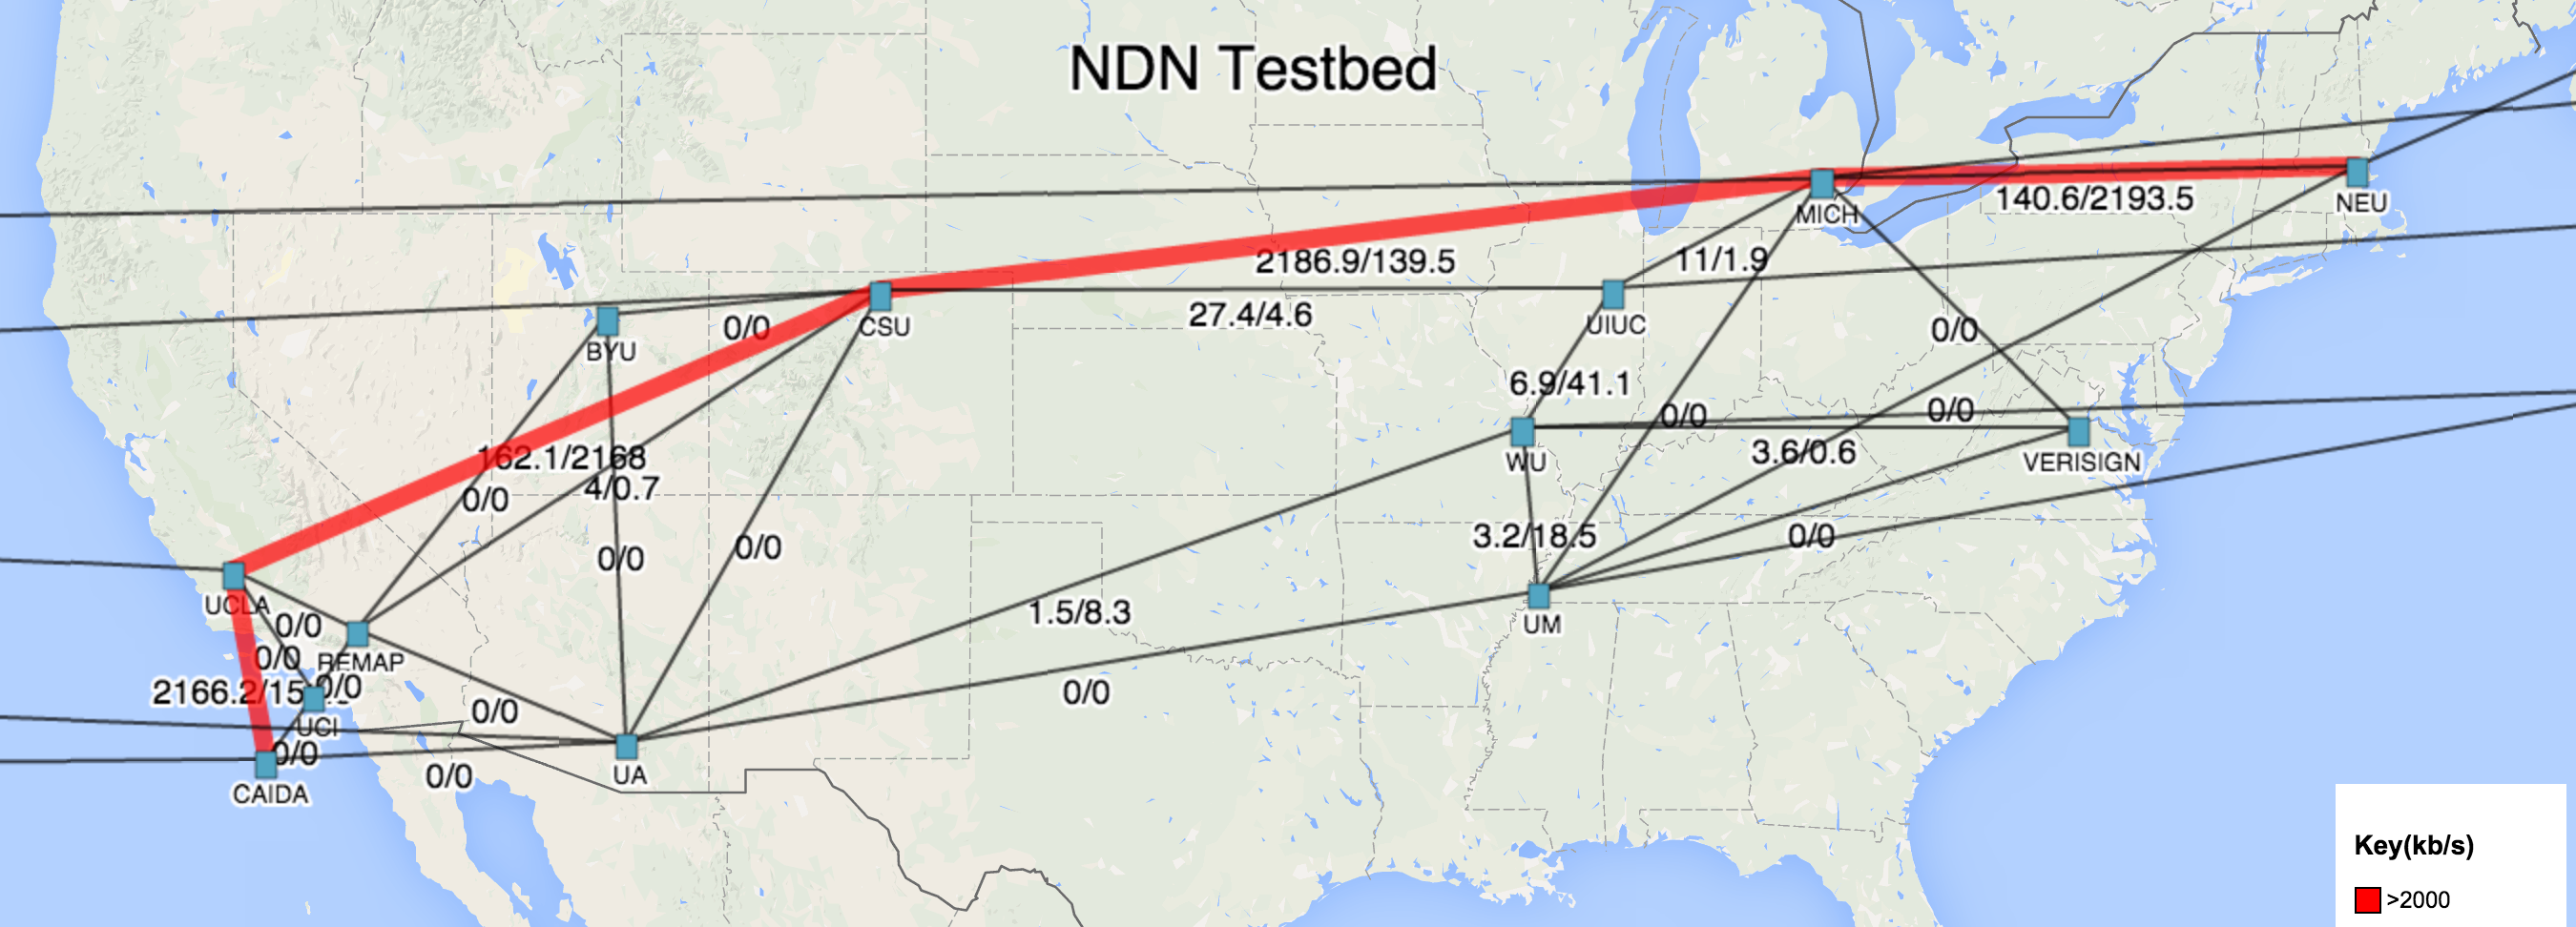
\includegraphics[scale=0.35]{ndnlive_6hops}
  % \vspace{-0.3cm}
  \caption{Overload Map over NDN Testbed}
  \label{fig:NDNlive_6hop}
  %\vspace{-0.2cm}
\end{figure*}

%\paragraph{Synchronization of video and audio} % (fold)
%\label{par:synchronization_between_video_and_audio}
%\vspace{0.3cm}
%There also exists the synchronization problem between video and audio. As we describe above~\ref{par:sync}, the Gstreamer will handle the synchronization part as long as we give the video and audio frame correct timestamps. In NDNlive, it is the capturing component who stamps the frames. In NDNtube, it is the \textit{Dumxer} who is responsible for time stamping. Once the media data flows through \textit{Dumxer}, this component will separate the video stream and audio stream according to their file type such as \textit{MP4} and adding the time information in each \textit{GstBuffer}.

  


% paragraph synchronization_between_video_and_audio (end)

% section implementation (end)